\documentclass[11pt,a4wide]{article}
\usepackage{verbatim}
\usepackage{listings}
\usepackage[pdftex]{graphicx}
\usepackage{a4wide}
\usepackage{color}
\usepackage{amsmath}
\usepackage{amssymb}
\usepackage[dvips]{epsfig}
\usepackage[T1]{fontenc}
\usepackage{cite} % [2,3,4] --> [2--4]
\usepackage{shadow}
\usepackage{hyperref}

\setcounter{tocdepth}{2}

\lstset{language=c++}
\lstset{basicstyle=\small}
\lstset{backgroundcolor=\color{white}}
\lstset{frame=single}
\lstset{stringstyle=\ttfamily}
\lstset{keywordstyle=\color{red}\bfseries}
\lstset{commentstyle=\itshape\color{blue}}
\lstset{showspaces=false}
\lstset{showstringspaces=false}
\lstset{showtabs=false}
\lstset{breaklines}
\begin{document}
\section*{Project 3}
\section*{Evan Markel}

My C++ program is located here in GitHub \url{https://github.com/evanmarkel/Project3}

\section*{Introduction}
%
In this project, I have used numerical methods to solve second order differential equations to simulate the solar system. Using relative units for distance, velocity, and mass, I was able to discretize the equations in unitless quantities similar to previous projects. The Runge-Kutta4 method and Verlet algorithm have proven very accurate in modeling celestial dynamics according to Newton's and Kepler's laws. We begin by separating Newton's second law of motion into into its two-dimensional Cartesian components for a circular orbit here: 
\[
\frac{d^2x}{dt^2}=\frac{F_{G,x}}{M_{\mathrm{Earth}}},
\]
and 
\[
\frac{d^2y}{dt^2}=\frac{F_{G,y}}{M_{\mathrm{Earth}}},
\]\newline
We then can use these equations along with the equation for force below to derive four coupled first order differential equations for celestial motion in two-dimensions. 
\[
F_G= \frac{M_{\mathrm{body1}}v_{body1}^2}{r}=\frac{GM_{body2}M_{\mathrm{body1}}}{r^2},
\]\newline
We then express the motion of body 1 around body 2 with four component time derivatives: 
\[
\frac{dv_{x1}}=\frac{-G*M_{body2}}{r^{3}}*x_{body1}, \hspace{.5} \frac{dx_{body1}}{dt}=v_{x}_{body1}
\]
and
\[
\frac{dv_{y1}}=\frac{-G*M_{body2}}{r^{3}}*y_{body1}, \hspace{.5} \frac{dy_{body1}}{dt}=v_{y}_{body1}
\]
The above equations now become the and utilizing the numerical Verlet, Euler-Cromer, and Runge-Kutta algorithms to solve the differential equations pertaining to the time derivatives in the physical laws. 

\newpage
\begin{enumerate}
\item[\bf Two-Body Problem]
These equations nicely predict the motion of the earth around the sun in my simulation. My code creates a celestial object which generates a vector in the SolarSystem class that contains the initial position and velocity for the object in two dimensions. For the Earth, we can easily find the needed initial velocity for circular motion: 
\[
v_{earth}^2r=GM_{\odot}=4\pi^2\mathrm{AU}^3/\mathrm{yr}^2.
\]\newline
For $r=1AU$ we see that in these units $v_{earth}=2*\pi$. Using this velocity and initial position of (1AU,0) we get a stable orbit. 
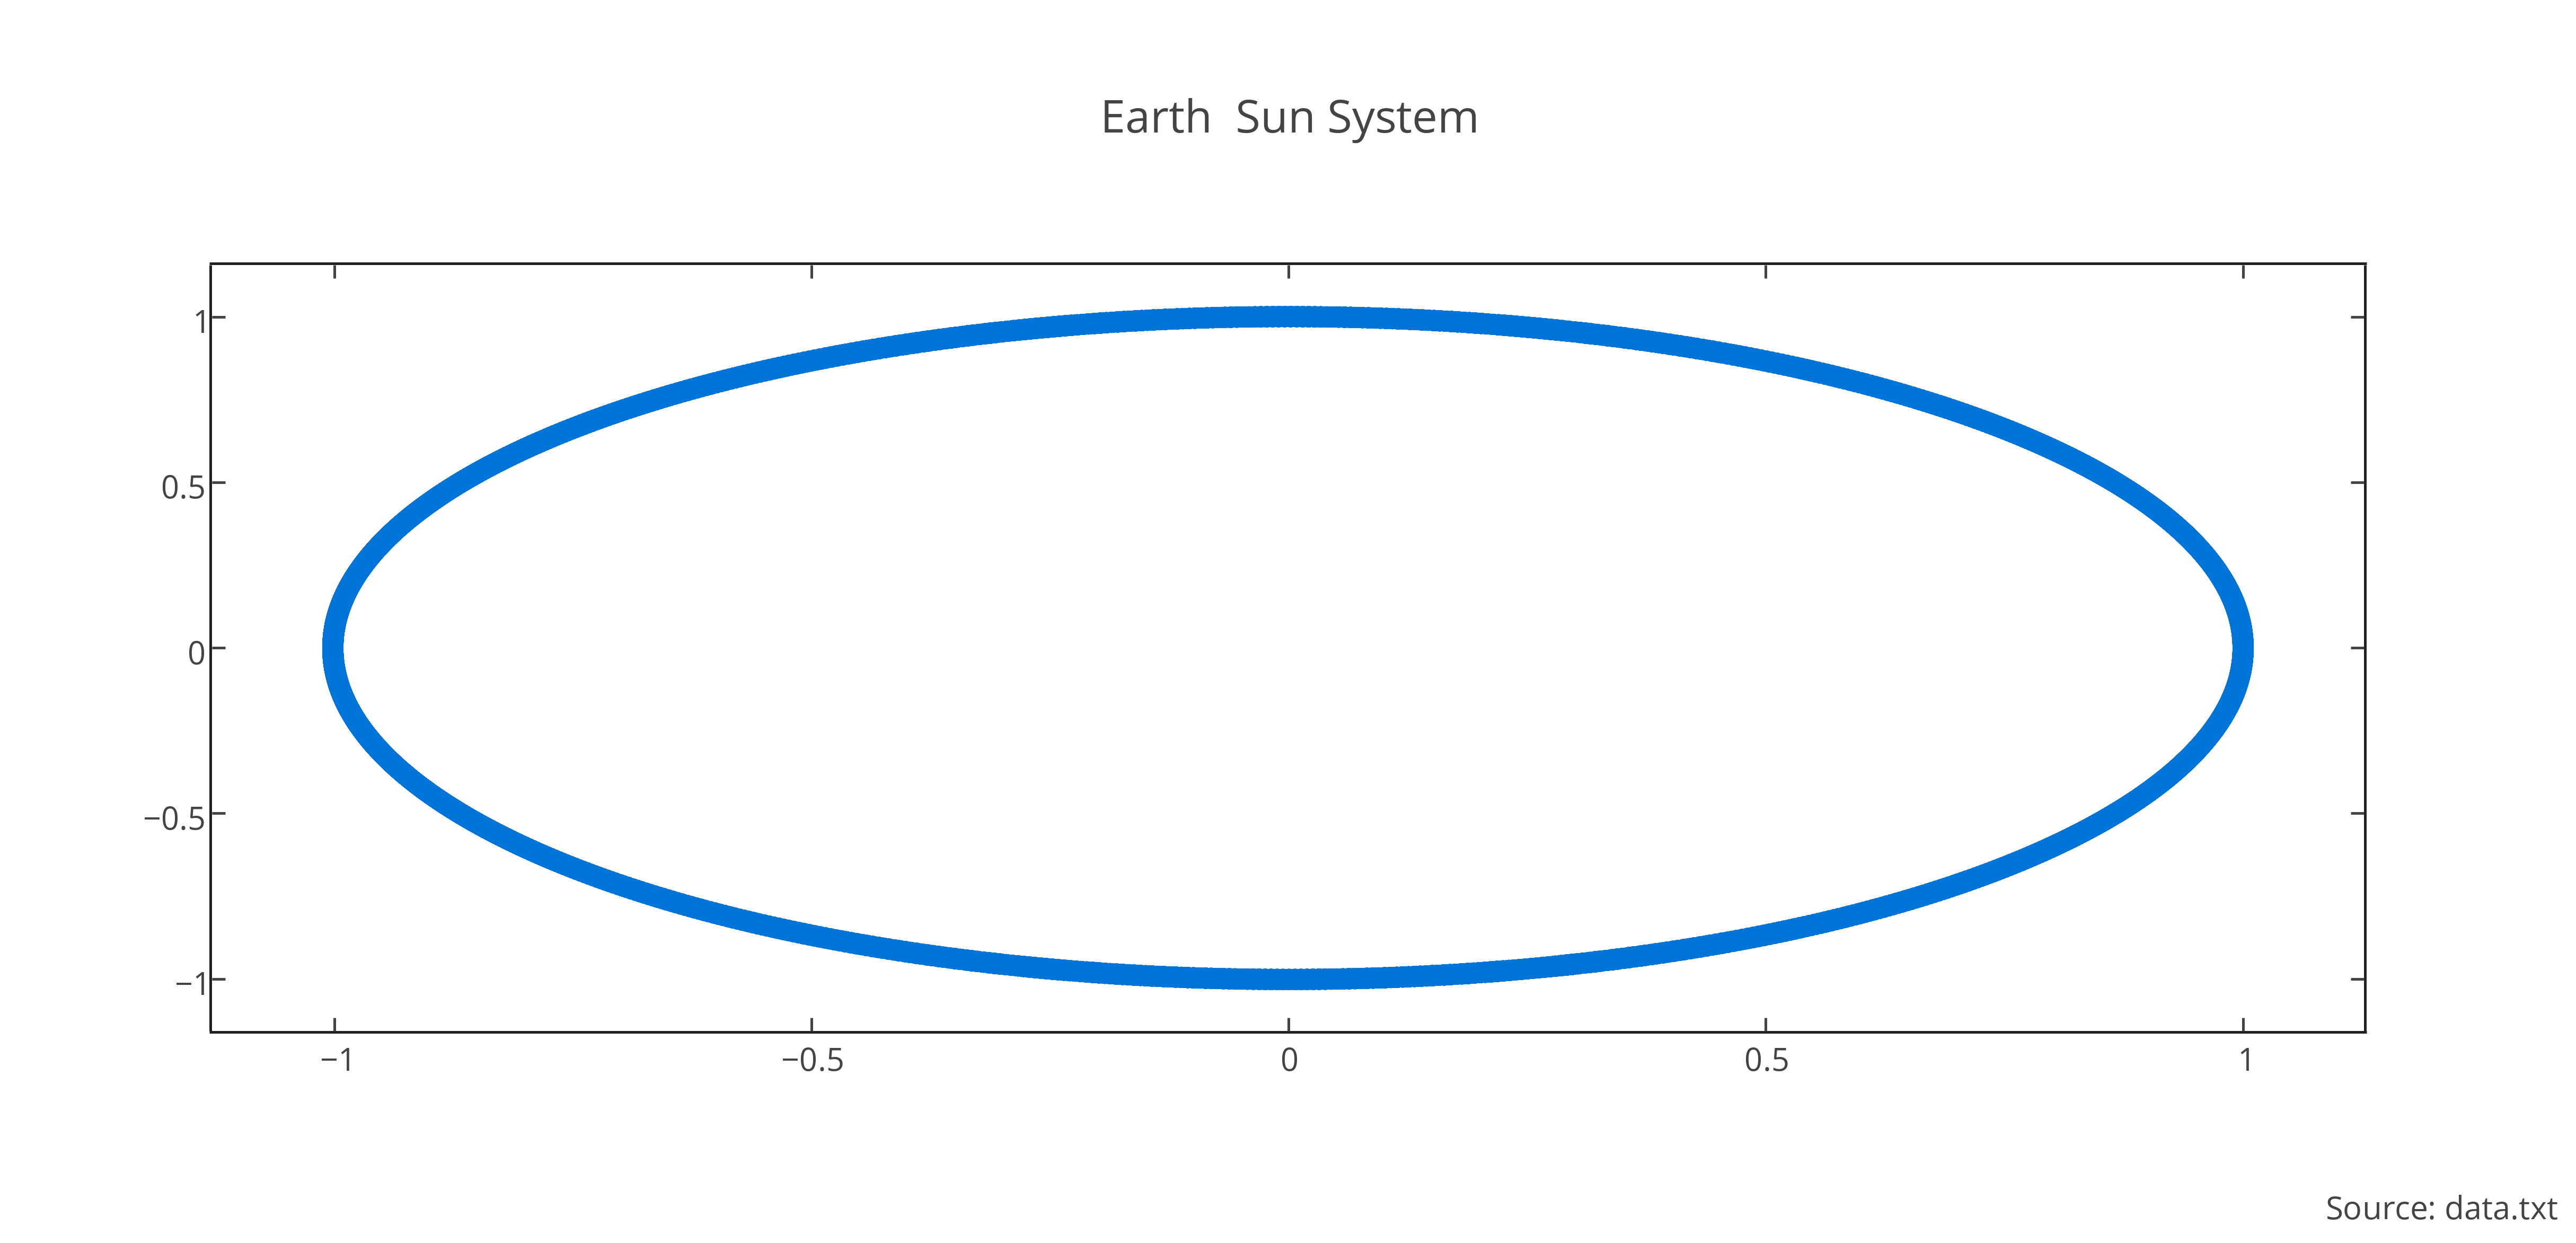
\includegraphics[width=6in,height=4.5in]{earth_sun_system.png}//
\item[\bf Part B]
Comparing my eigenvalues with the Armadillo $eig_sym(A)$ solver yielded nearly identical results for larger values of N. The eigenvalues also correspond to the correct energy states (3,7,11, etc) as given in the project description, so we can go on to the more complicated problem knowing the algorithm works.The numerical values are given in the table below. \newline
After running my algorithm, the parameters $N_step$ and $\rho_{max}$ need to be decided upon before moving to the two electron wave equation. First, here's a table showing the number of steps given to the algorithm in order to determine four leading digits for the first 3 eigenvalues. For this case, our $\epsilon = 1e-8$, which is the low level threshold for assigning non-diagonal matrix elements as essentially zero. Also, $\rho_{max} = 5$ for this table.  
\begin{center}
    \begin{tabular}{| c | c | c | c | c |}
    \hline
    \bf$ N_{step}$	& \bf $\lambda_{1}$	 & $\bf \lambda_{2}$	 & $\bf \lambda_{3}$	 & 	\bf No. iterations \\ \hline
	10 & 2.9338	 & 6.6598 &  10.1415 & 139 \\ \hline
	50 & 2.9970  & 6.9850  & 10.963 & 4,039 \\ \hline
	100 & 2.9992 & 6.9962 & 10.991 & 16,474 \\ \hline
	125 & 2.9995 & 6.9975 & 10.994 & 25,826 \\ \hline
	150 & 2.9997 & 6.9983  & 10.996 & 37,443 \\ \hline
	175 & 2.9997 & 6.9987 	& 10.997 & 50,991 \\ \hline
	200 & 2.9998 & 6.9990 	& 10.998 & 66,827 \\ \hline
	225 & 2.9998 & 6.9992	& 10.998 & 84,775 \\ \hline
	250 & 2.9999 & 6.9994 	& 10.999 & 104,290 \\ \hline
	275 & 2.9999 & 6.9996 	& 10.999 & 128,507 \\ \hline
	400 & 3.0000 & 6.9998 	& 11.000 & 269,020 \\ 
	 \hline	
    \end{tabular}
\end{center}

Using $N_{steps}$ =250 gives us (basically) four leading digits and the values of $\epsilon$ and $\rho_{max}$ are good choices as well. These are the values I use throughout the project. However, just to check: when I change $\rho_{max}$ to 10, and $N_{steps}$ =100, the values are $\lambda_{1}$ = 2.9969, $\lambda_{2}$ = 6.9846, and $\lambda_{3}$ = 10.962. The relative error compared with the table above for n=100 are $.077\%$ for $\lambda_{1}$, $.165\%$ for $\lambda_{2}$, and $.264\%$ for $\lambda_{3}$. When $\rho_{max}$ = 100, the results are very far off. Since this is a numerical estimation, a lower value for  $\rho_{max}$ gives a more accurate solution. However, $\rho_{max}$ must be large enough to give us a good physical picture. 
Here is a graph of the $N_{step}$ -the dimensionality of the matrix versus the number of iterations needed to get the eigenvalues. We can see that it goes$\sim O(n^{2})$.
\includegraphics[width=6in,height=4.5in]{iterations.png}//
Now we'll look at the run-time of the Jacobi method versus the the armadillo solver. The values :$\epsilon$=1e-8 and $\rho_{max}$ =5.  
\begin{center}
    \begin{tabular}{| c | c | c |}
    \hline
   \bf $N_{step}$ & \bf Armasolve time	 & \bf Jacobisolve time \\ \hline
	10 & .00071311	 & $7.4863 x 10^{-5}$  \\ \hline
	50 & .00955606 & .021553   \\ \hline
	100 & .119834 & .297856 \\ \hline
	150 & .292907 & 1.43716   \\ \hline
	200 & .543296 & 4.43368  \\ \hline
	250 & .854114 & 10.6005	 \\ \hline
	400 & .879044 & 73.0668	 \\ 
	 \hline	
    \end{tabular}
\end{center}
We see that the Jacobi is actually faster for N=10 but then gets much slower as N increases into the range that we need for numerical precision. 


\item[\bf Part C]
We now move on to the two electron case. The main difference here is the change in potential. The Schr\"odinger equation simplifies as in part a as follows: 
\[
  -\frac{d^2}{d\rho^2} \psi(\rho) 
       + \frac{1}{4}\frac{mk}{\hbar^2} \alpha^4\rho^2\psi(\rho)+\frac{m\alpha \beta e^2}{\rho\hbar^2}\psi(\rho)  = 
\frac{m\alpha^2}{\hbar^2}E_r \psi(\rho) .
\]
The change in potential from a goes as $\rho^2$ to $\omega_r^2\rho^2+1/\rho$. The $\omega_r$ term indicates the strength of the oscillator potential and will influence the values of the energy states of the two particle system. We look at the cases where $\omega_r = 0.01$, $\omega_r = 0.5$, $\omega_r =1$, and $\omega_r = 5$.  We change the potential and re-run the program for the 4 different values of $\omega_r$. The first 3 eigenvalues are given in the table below. The results use $N_{step}$ at 250, $\rho_{max}$ at 5, and $\epsilon$ at 1e-8. 
\newline
\begin{center}
    \begin{tabular}{| c | c | c | c |}
    \hline
    \bf $\omega_r$	& \bf  $\lambda_1$	 & \bf  $\lambda_{2}$ & \bf  $\lambda_{3}$ \\ \hline
	0.01 & 0.84075	 & 2.1737 &  4.2372\\ \hline
	0.5 & 2.2310 & 4.1691  & 6.3858 \\ \hline
	1.0 & 4.0577 & 7.9091 & 11.818\\ \hline
	5.0 & 17.445 & 37.057 & 56.817 \\ 
	 \hline	
    \end{tabular}
\end{center}
Here are the values for the first 3 energy states. We see the dependence on $\omega_r$ is quite large for the values of the energy levels. For $\omega_r$ = .01, the electrons are not closely coupled and the energy level of the oscillator is even lower than for the single electron case. We see when $\omega_r$ grows to 1 and 5, the values are higher. Physically, the electrons are brought closer together in the oscillator well and the repulsive force means that the energy needed for the state to exist is greater. The greater potential should lead to a higher value of the eigenvalues. 

\item[\bf Part D]
Finally, we want to plot the wave functions for the first 3 energy states for the 4 $\omega_r$ values. The eigenvectors contain the constituent elements of the wave equation at the various positions along $[0,\rho_{max}=5.0]$. The tricky part is indexing the locations of the eigenvectors within the eigenmatrix from the position of the corresponding eigenvalue. Since the Jacobi algorithm does not necessarily return the eigenvalues in sorted order, another for loop is needed to extract the first 3 eigenvectors--> corresponding to the 3 lowest energy states. \newline
The next tricky part is determining how to normalize the eigenvectors. From quantum mechanics, we know that in an infinite potential well, the wave function should be normalized by $sqrt(2/length of well)$. In our case, we have abstracted the parameters in this assignment, and therefore the normalization is a bit more abstract here. There should be an h term-or a similar term that takes into account the length of the well- included in the normalization. While this may be a concern, the probability distribution function is the square of the wave equation and must sum to 1. Therefore, any constant in front of the wave equation can be eliminated as it will not change the relative values of the wave equation when multiplied uniformly. And since we are normalizing to 1, the term can be omitted. So in my code, I've squared the eigenvectors and applied the armadillo normalise() function.  I've included 4 plots for the 4 different values of $\omega_r$. The first 3 eigenvectors are graphed on top of each other in each case to highlight the relative probability strengths. 
\includegraphics[width=6in]{w=001.png}\\
\includegraphics[width=6in]{w=05.png}\\
\includegraphics[width=6in]{w=10.png}\\
\includegraphics[width=6in]{w=50.png}\\
We can see the coupling effect of the oscillator strength. The electron can spread out more freely with lower $\omega_r$ values and is more tightly bound for higher ones. The shape of the distribution functions seems correct and the strong and weak particle interactions due to the strength of the harmonic oscillator as $\omega_r$ are also apparent from the plots. The area under the curve for each of the 3 energy states sum to 1. The peaks for the energy states 2 and 3 have higher probabilities closer to zero for $\omega_r$= .01  and this is reversed for $\omega_r$ = 0.5, 1.0, and 5.0. I have some reservations about the correctness of the eigenvector plots, but here's my hand-waving attempt: I imagine the probability of the smaller relative radius would be greater for a weaker harmonic oscillator coupling than for a stronger one. Based on these plots, I conjecture that the higher $\omega_r$ means a more tightly bound nucleus with the electrons pushing more towards the outside of the well (Coulomb repulsion) which is a result of the higher potential energy of that system.The lower $\omega_r$ strength has a higher entropy and lower energy than the higher $\omega_r$ strengths. We can also see this higher cost energy effect in the relative growth of the first 6 eigenvalues as plotted below in a stacked area chart divided by the four oscillator strengths: 
\includegraphics[width=6in]{eigenvaluesw.png}

\item[\bf Conclusion]

This project has interesting physical takeaways and demonstrates how some simple algorithms can aid a great deal toward solving problems where there is no easy analytical solution. 

\end{enumerate}


\end{document}

